\chapter{Dal progetto al codice}


\section{Trasformare i progetti in codice}

\dfn{Modello di implementazione}{
    Un \newfancyglitter{modello di implementazione} è costituito da tutti gli
    elaborati dell'implementazione, come il \newfancyglitter{codice sorgente},
    la definizione delle \newfancyglitter{basi di dati}, le pagine
    JSP/XML/HTML, etc.
}

\begin{itemize}
    \item [$\Rightarrow$] L'implementazione è un processo di traduzione
    relativamente meccanico del progetto in codice;
    \item [$\Rightarrow$] Ci possono essere dei cambiamenti e delle deviazioni
    rispetto al progetto originale.
\end{itemize}

\nt{Java viene utilizzato come linguaggio di esempio, ma i concetti sono
applicabili a qualsiasi linguaggio di programmazione OO.}

\ex{Traduzione}{
    \begin{center}
        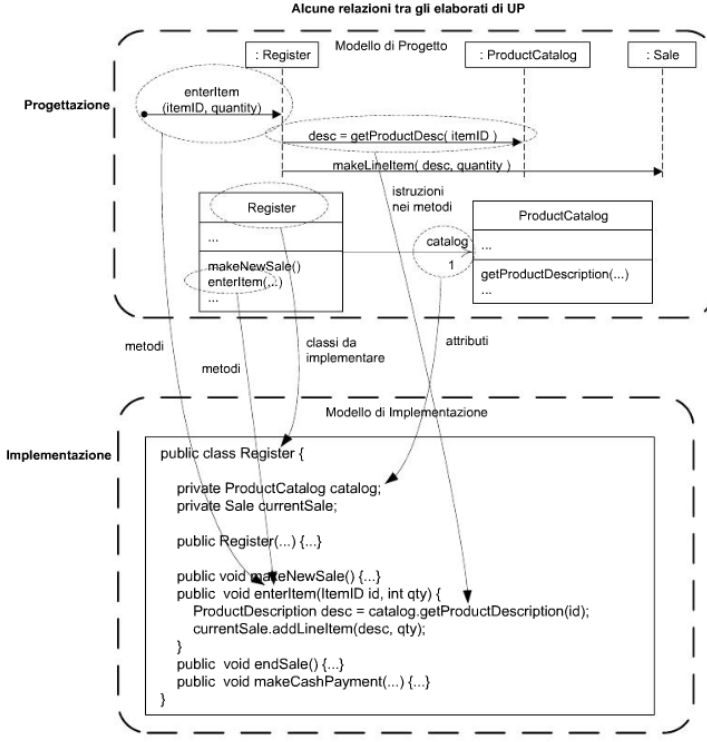
\includegraphics[scale=0.3]{images/Implementazione.png}
    \end{center}
}

\ex{Traduzione di attributi e firme}{
    \begin{center}
        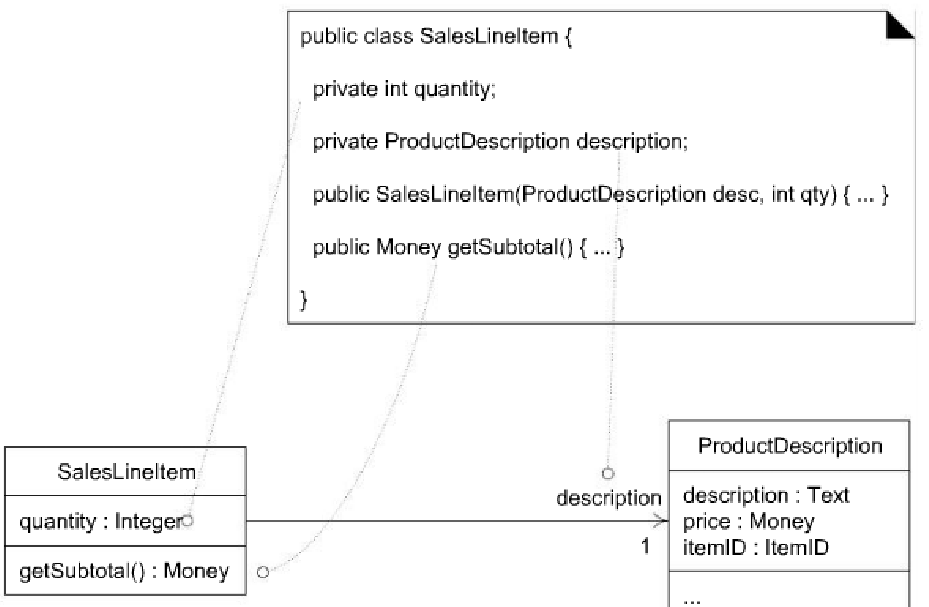
\includegraphics[scale=0.3]{images/TraduzioneAttributiFirme.png}
        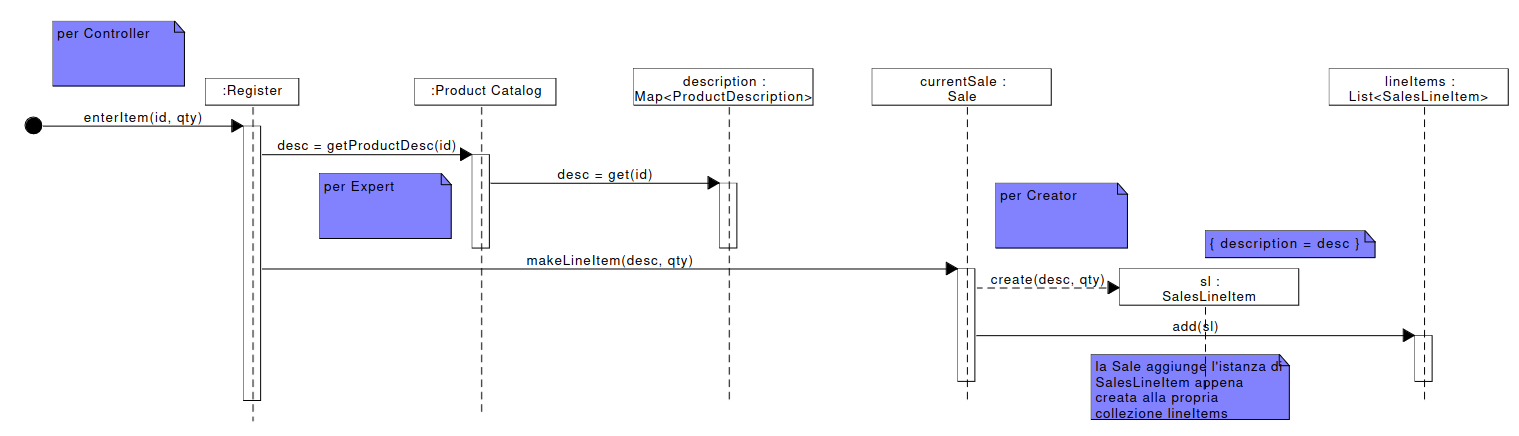
\includegraphics[scale=0.3]{images/TraduzioneAttributiFirme2.png}
    \end{center}

}

\subsection {Collezioni e costruttori}

\dfn{Collezione}{
    Una \newfancyglitter{collezione} è un contenitore di oggetti, che può
    essere usato per memorizzare, recuperare e manipolare dati.
}

\nt{Le relazioni uno a molti sono generalmente implementate tramite
collezioni.}

\ex{Associazioni}{
    \begin{center}
        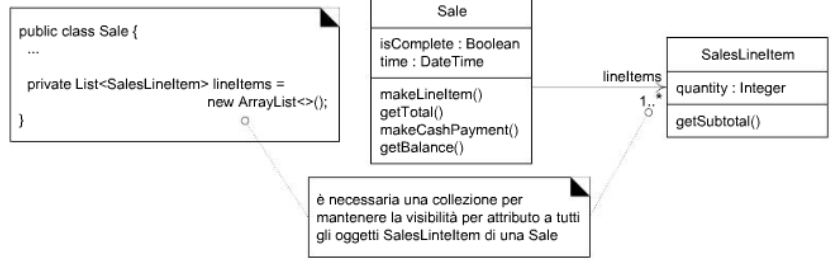
\includegraphics[scale=0.5]{images/Associazioni.png}
    \end{center}
}

\dfn{Costruttore}{
    Un \newfancyglitter{costruttore} è un metodo speciale che viene invocato
    quando un oggetto viene creato.
}

\begin{itemize}
    \item [$\Rightarrow$] I costruttori possono venir scritti per ispezione
    da un diagramma delle classi.
\end{itemize}

\ex{Costruttori}{
    \begin{center}
        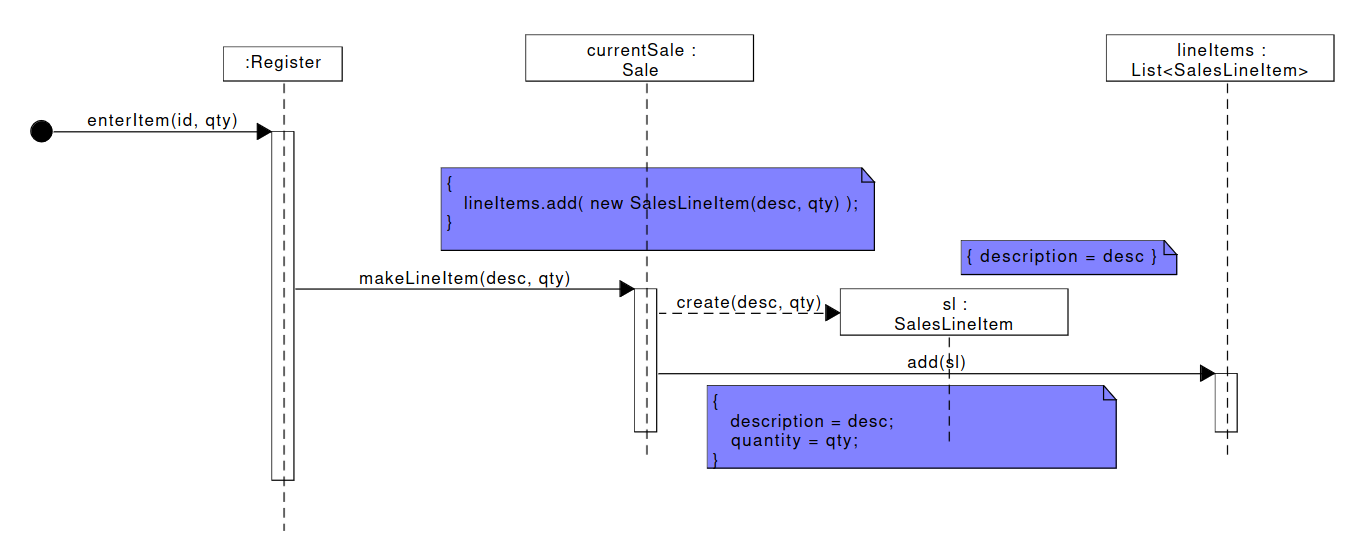
\includegraphics[scale=0.3]{images/Costruttori.png}
    \end{center}
}

\subsection{Ordine di implementazione}

\begin{itemize}
    \item [$\Rightarrow$] Le classi possono essere implementate in modo e 
    ordine diversi (es. dalla meno accoppiata alla più accoppiata).
\end{itemize}

\ex{Ordine di implementazione}{
    \begin{center}
        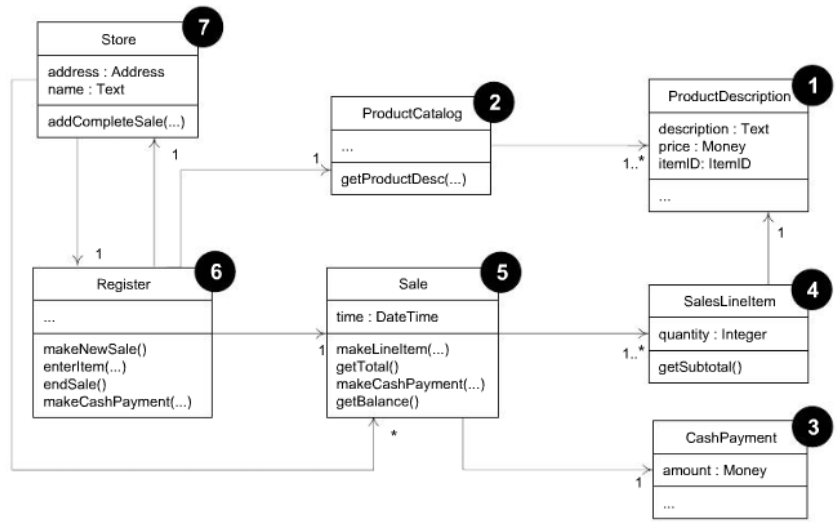
\includegraphics[scale=0.5]{images/OrdineImplementazione.png}
    \end{center}
}

\section{Sviluppo test-driven e refactoring}

\subsection{I test}

\begin{itemize}
    \item [$\Rightarrow$] XP ha promosso la \fancyglitter{pratica dei test}:
    si scrivono i test prima di scrivere il codice.
\end{itemize}

\dfn{Test-Driven Development (TDD)}{
    Il \newfancyglitter{Test-Driven Development} è una pratica di sviluppo
    software che prevede la scrittura dei test prima di scrivere il codice.

}

\nt{Si immagina che il codice sorgente sia già stato scritto e si scrivono
i test che si aspettano che il codice passi.}

\paragraph{Vantaggi:}

\begin{itemize}
    \item [\textcolor{dkgreen}{\checkmark}]  La soddisfazione del programmatore
    porta a una scrittura più coerente dei test;
    \item [\textcolor{dkgreen}{\checkmark}]  L'interfaccia e i comportamenti
    sono più chiari;
    \item [\textcolor{dkgreen}{\checkmark}] La verifica è dimostrabile,
    ripetibile e automatizzabile;
    \item [\textcolor{dkgreen}{\checkmark}] Si ha maggiore fiducia nei cambiamenti.
\end{itemize}

\paragraph{Ci sono diversi tipi di test:}

\begin{itemize}
    \item [$\Rightarrow$] \fancyglitter{Test unitari}\footnote{Visti in "Algorimi e strutture dati"}: testano singole unità di codice;
    \item [$\Rightarrow$] \fancyglitter{Test di integrazione}: testano la comunicazione tra specifiche parti;
    \item [$\Rightarrow$] \fancyglitter{Test end-to-end}: testano l'intero sistema;
    \item [$\Rightarrow$] \fancyglitter{Test di accettazione}: testano il sistema, considerandolo a scatola nera, dal punto di vista dell'utente (con riferimento ai Casi d'Uso).
\end{itemize}

\paragraph{I test unitari sono composti da quattro fasi:}

\begin{enumerate}
    \item \fancyglitter{Preparazione}: si ccrea l'oggetto (o il gruppo di
    oggetti) da testare (\textit{fixture}) e si preparano altri oggetti e/o risorse necessarie per i test;
    \item \fancyglitter{Esecuzione}: si fa fare qualcosa alla fixture, viene richiesto un comportamento specifico;
    \item \fancyglitter{Verifica}: si verifica che i risultati ottenuti siano 
    quelli attesi;
    \item \fancyglitter{Rilascio}: si rilascia la fixture e si puliscono le risorse (per evitare la corruzione di altri test).
\end{enumerate}

\subsection{Il refactoring}

\nt{Gli sviluppi incrementali degradano la qualità del codice.}

\begin{itemize}
    \item [$\Rightarrow$] XP ha promosso il \fancyglitter{refactoring continuo}:
    si modifica il codice per renderlo più chiaro e più semplice da capire,
    con meno duplicazioni.
\end{itemize}

\dfn{Refactoring}{
    Il \newfancyglitter{refactoring} è un metodo strutturato e disciplinato per scrivere o 
    ristrutturare del codice esistente, senza cambiarne il comportamento esterno.
    Si applicano piccoli passi di trasformazione in combinazione con i test a ogni passo.
}

\cor{Refactoring e test}{
    Dopo ciascuna trasformazione, si eseguono i test unitari per verificare che
    il refactoring non abbia provocato una \fancyglitter{regressione} (fallimento).
}

\paragraph{Regole per TDD e refactoring:}

\begin{enumerate}
    \item Si scrive un test unitario che fallisce per dimostrare
    la mancanza di una funzionalità o di codice;
    \item Si scrive il codice per far passare il test;
    \item Si riscrive o ristruttura il codice, migliorandolo oppure si
    passa al prossimo test unitario.
\end{enumerate}

\begin{center}
    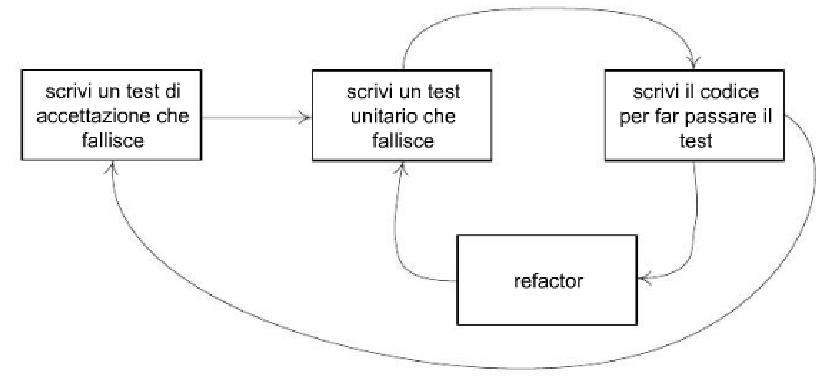
\includegraphics[scale=0.35]{images/Test.png}
\end{center}

\paragraph{Gli obiettivi del refactoring sono:}

\begin{itemize}
    \item [$\Rightarrow$] Migliorare la leggibilità del codice;
    \item [$\Rightarrow$] Eliminare il codice duplicato;
    \item [$\Rightarrow$] Eliminare l'uso dei letterali costanti hard-coded;
    \item [$\Rightarrow$] Abbreviare i metodi lunghi.
\end{itemize}

\begin{center}
    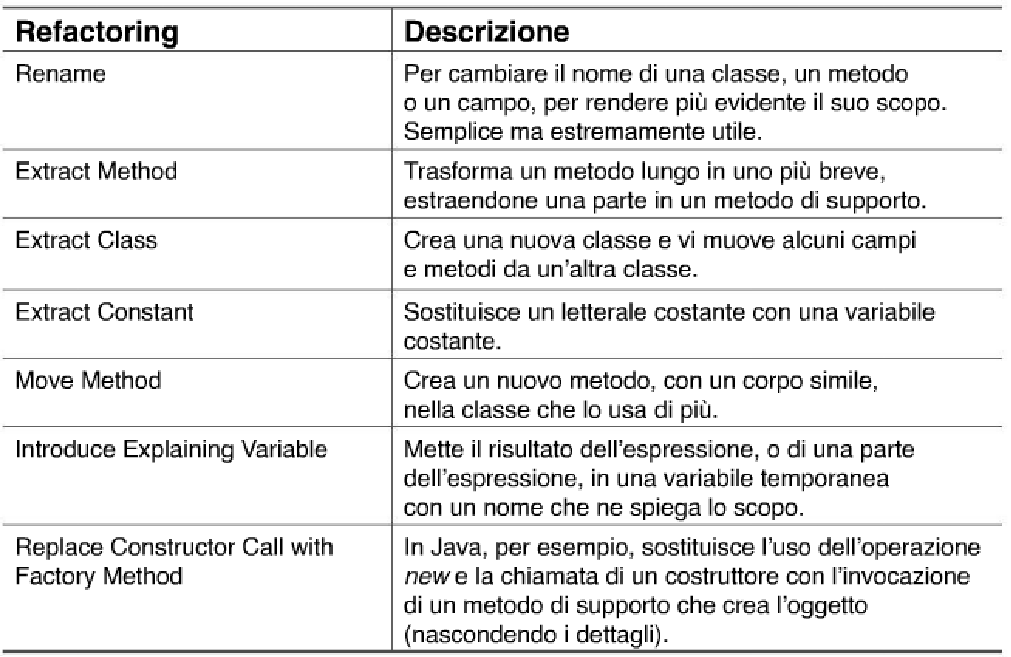
\includegraphics[scale=0.4]{images/Refactoring.png}
\end{center}